\documentclass[a4paper,titlepage,12pt]{scrreprt}

\usepackage{ucs}
\usepackage[utf8x]{inputenc}
\usepackage[T1]{fontenc}
\usepackage[ngerman]{babel}
\usepackage{datetime}
\usepackage{amssymb}
\usepackage[hidelinks]{hyperref}
\usepackage{amsmath}
\usepackage{graphicx}
\usepackage{color}
\usepackage{titling}
\usepackage[figure]{hypcap}
\usepackage{subcaption}
\usepackage{tabularx}
\usepackage{eso-pic} % for aligning the title page figures
\usepackage[official]{eurosym} % for €
\usepackage{units} % for correct spacing when using units

% Zeilenabstand ----------------------------------------------------------------
\usepackage{setspace}
\onehalfspacing  % 1,5 Zeilen (entspricht ang. dem doppelten Zelenabstand in Word)
\frenchspacing   % Kein doppeltes Leerzeichen nach '.' etc.

% Schusterjungen und Hurenkinder -----------------------------------------------
% Hiermit werden Schusterjungen und Hurenkinder verhindert
% Zur Info:
% http://de.wikipedia.org/wiki/Hurenkind_und_Schusterjunge
\clubpenalty = 10000
\widowpenalty = 10000
\displaywidowpenalty = 10000

% Seitenlayout --------------------------------------------------------------------
\usepackage{geometry}
\usepackage{vmargin}
\setmarginsrb{35mm}{20mm}{25mm}{20mm} % 
			 {7mm}{15mm}{4mm}{20mm}
			 
% Datum ------------------------------------------------------------------------
%	Diese Definition wird benötigt um auf der Titelseite nur Monat und Jahr aus-
%	zugeben.
\usepackage{datetime}
\newdateformat{titledate}{\monthname[\THEMONTH] \THEYEAR}
			 
\allowdisplaybreaks

% ------------Definitionsbereich------------ %

% zum Referenzieren
\newcommand{\refchapter}[1]{Kapitel~\ref{#1}}
\newcommand{\refsec}[1]{Abschnitt~\ref{#1}}
\newcommand{\reffig}[1]{Abbildung~\ref{#1}}
\newcommand{\reftab}[1]{Tabelle~\ref{#1}}

% --------------Dokumenteinstellungen------------- %

% Schriftart: 
% - https://en.wikibooks.org/wiki/LaTeX/Fonts#Font_styles
% - https://de.overleaf.com/learn/latex/Font_typefaces#Reference_guide
\usepackage{tgadventor}

% --------------Dokumentanfang------------- %

\begin{document}

% Titel
\newdateformat{mydate}{\monthname[\THEMONTH] \THEYEAR}

\begin{titlepage}

    \AddToShipoutPictureBG*{\AtPageUpperLeft{\makebox[\paperwidth][l]{\raisebox{-\height}{
\includegraphics[width=7.5cm]{../figures/TOSLogo.png}}}}}
    \AddToShipoutPictureBG*{\AtPageUpperLeft{\makebox[\paperwidth][r]{\raisebox{-\height}{
\includegraphics[width=7.5cm]{../figures/COSIMALogo.png}}}}}
    
    \small
	\parindent0pt
	
	\begin{center}
		\bfseries Projektmappe für den COSIMA-Wettbewerb 2018
	\end{center}
	\vspace*{15mm}
	\normalsize	
	\begin{center}
		\huge
		{\bfseries\sffamily Der Gestikulaser}
		\\ \vspace*{4mm}
		\large
		Die neue Technologie der Gestenerkennung
	\end{center}
	\vfill
	\begin{center}
	\large \mydate{\today}
	\end{center}
	
\includegraphics[width=15cm,height=9cm]{../figures/GestikulaserLogo.png}
	\vfill
	\begin{center}
		Verfasst von \\[3ex]
		Christoph Behr \\
		Cailing Fu \\
		Nicole Grubert \\
		Daniel Wolff \\
	\end{center}
\end{titlepage}

% Inhaltsverzeichnis
\tableofcontents
\newpage

% Einführung
\chapter{Einleitung}
\label{ch:Einleitung}

\textcolor{red}{Was wurde gemacht? Was war die Motivation? Inwiefern besitzt das Projekt eine Alltagsrelevanz?}

Gestenerkennung ist immer wieder ein Thema, welches viel Aufmerksamkeit erregt. Und obwohl ein Mensch recht einfach verschiedene Gesten erkennen kann, ist es für den Computer eine große Herausforderung, zuverlässig die Gesten eines Menschen zu erkennen. \\
Mit dem Gestikulaser wollen wir ein neues System entwickeln, um Handgesten eines Menschen zu erkennen. Dabei soll dieses nicht mit einer Kamera arbeiten, wie die meisten heute verfügbaren Systeme, sondern die Hand des Nutzers soll mit Infrarot-LEDs beleuchtet und die Gesten sollen durch die erzeugten Reflektionsmuster erkannt werden. Eine auf diese Weise realisierte Gestenerkennung ist nicht nur Tageslicht unabhängig, sondern kann auch in vollkommener Dunkelheit betrieben werden. \\
Mit Hilfe eines modularen Stecksystems aus mehreren Komponenten soll es möglich sein, ein individuelles Muster des Systems anzufertigen. Somit soll in Zukunft nicht nur die Handgesten-Steuerung möglich sein, sondern auch eine Ganzkörper-Gestensteuerung wie sie in einer Cave verwendet werden könnte, ermöglicht werden. \\

Im Alltag kann der Gestikulaser eingesetzt werden, um verschiedenste Dinge, wie ein ferngesteuertes Auto, eine Smart Home Einrichtung oder eine Drohne zu steuern. 
\chapter{Stand der Technik}
\label{ch:StandDerTechnik}

Mit dem zunehmenden Einfluss von Computern auf die Gesellschaft wurde auch die Interaktion von Mensch und Computer ein immer wichtigerer Bestandteil unseres Alltags. Innerhalb der letzten Jahrzehnte wurde auf diesem Gebiet stetig geforscht und die verfügbaren Technologien weiterentwickelt, mit dem Ziel, die Interaktion von Mensch und Computer so natürlich wie möglich zu gestalten. Diese Entwicklung erstreckte sich von der ursprünglichen Kommunikation mittels Maus und Tastatur, über Touchscreens und Virtual Reality Systeme, bis hin zu Sprachsteuerungen von elektronischen Endgeräten. Vor diesem Hintergrund hat auch das Interesse an Gestenerkennung als zusätzliches natürliches Kommunikationsmittel zugenommen. \\
Bei Gestenerkennungssystemen kann man grundsätzliche zwischen zwei verschiedenen Arten von Gestenerkennung unterscheiden: Bei der \textit{gerätebasierten Gestenerkennung} werden die Bewegungen eines Nutzers durch Beschleunigungs- oder Positionssensoren wahrgenommen und einer Geste zugeordnet. Bei dieser Art der Gestenerkennung muss der Nutzer die Sensorik in irgendeiner Form am Körper tragen, damit die Bewegungsmuster richtig aufgezeichnet werden können. Dabei kann z.B. ein Handschuh wie z.B. der CyberGlove II des Unternehmens CyberGlove Systems (siehe auch \reffig{fig:CyberGlove}) oder ein einfacher Controller wie bei der Spielekonsole Wii von Nintendo (siehe \reffig{fig:WiiController}) zum Einsatz kommen.
\begin{figure}[h]
	\centering
	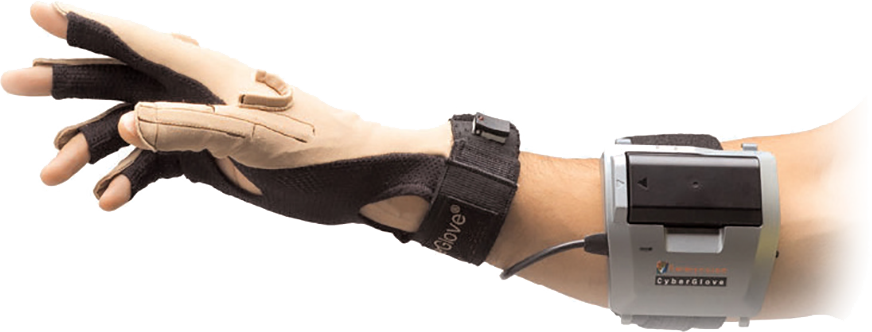
\includegraphics[scale=0.4]{../figures/CyberGlove.png}
	\caption{Der CyberGLove II von CyberGlove Systems. Er enthält verschiedene Sensoren, unter Anderem Biegesensoren für die Finger, sowie Sensoren zur Detektion der Drehung des Handgelenks. \source{\url{http://www.cyberglovesystems.com/cyberglove-ii/}}}
	\label{fig:CyberGlove}
\end{figure}
\begin{figure}[h]
	\centering
	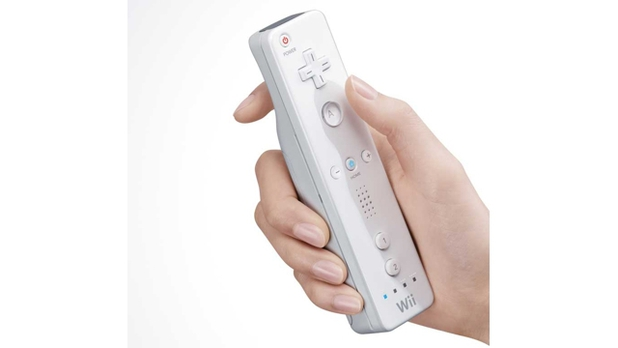
\includegraphics[scale=0.5]{../figures/WiiController.jpg}
	\caption{Ein Controller der Nintendo Spielekonsole Wii. Die Erkennung der Bewegungen des Spielers erfolgt mit Hilfe von Positions- und Beschleunigungssensoren. \source{\url{https://www.chip.de/artikel/Nintendo-Wii-Test-2_140216386.html}}}
	\label{fig:WiiController}
\end{figure}
\textit{Kamerabasierte Gestenerkennungsverfahren} nutzen externe Systeme, die die Bewegungen des Nutzers beobachten und Aufnahmen von dessen Bewegungsabläufen erstellen. Dabei werden meistens Kamerasysteme eingesetzt. Die aufgenommenen Bilddaten werden dann durch verschiedene Bildrekonstruktionsverfahren sowie Bildanalyseverfahren analysiert, um die Gestendaten zu extrahieren. Nachdem die Gestendaten extrahiert wurden, erfolgt ein Abgleich mit einer Datenbank, in der verschiedene Aufnahmen von verschiedenen Gesten gespeichert sind. Dieser Datenbankabgleich erlaubt letztendlich die Zuordnung der Geste. Ein Beispiel für ein System, das auf diese Weise arbeitet, ist die Kinect Erweiterung für die XBox-Spielekonsole von Microsoft (siehe auch \reffig{fig:MSKinect}).
\begin{figure}[h]
	\centering
	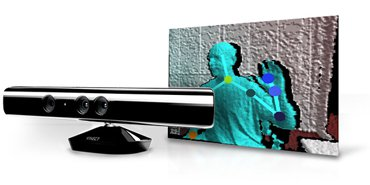
\includegraphics[scale=0.5]{../figures/MSKinect.jpg}
	\caption{Das kamerabasierte Gestenerkennungssystem Kinect von Microsoft. Es werden Aufnahmen des Nutzers gemacht, die nach einer Analyse mit einer Datenbank abgeglichen werden, um die Geste zu zuordnen. \source{\url{https://blogs.microsoft.com/ai/kinect-for-windows-game-on-for-commercial-use/}}}
	\label{fig:MSKinect}
\end{figure}
Beide Arten von Gestenerkennungssystemen werden aktuell eingesetzt. Allerdings haben beide Verfahren gewisse Nachteile: So erfordern gerätebasierte Gestenerkennungssysteme immer Sensorik am Körper des Nutzers, was sich in alltäglichen Situationen häufig als unkomfortabel erweist. 
Die kamerabasierte Gestenerkennungssysteme haben den Nachteil, dass
\begin{itemize}
	\item sie nur Gesten erkennen können, welche in der Datenbank vorhanden sind.
	\item Datenbankabfragen und Vergleiche mit den darin gespeicherten Daten sind häufig rechenaufwändig, was sich für die Echtzeit Erkennung der Gesten als problematisch erweisen kann.
	\item durch eine Anbindung an die Datenbank ständig Internet Zugang oder alternativ große Mengen an Speicherplatz benötigt wird. 
	\item je nach Auflösung nur grobe Gesten erkannt werden können..
	\item durch externe Vibrationen Probleme mit unscharfen Bildern entstehen können (wie zum Beispiel im Auto).
	\item sie bei Dunkelheit nicht arbeiten können. 
	\item sie Probleme mit der Bilderkennung haben, wenn die Hintergrundfarbe gleich der Hautfarbe ist. 
\end{itemize}
Insbesondere für den Einsatz in eingebetteten Systemen, wie z.B. in der Automobil-Industrie sind diese beiden Gestenerkennungsverfahren nur bedingt geeignet: Gerätebasierte Gestenerkennungssysteme benötigen externe Sensorik am Körper des Nutzers, die mit dem eingebetteten System kommunizieren und Daten austauschen muss. Dabei ist in eingebetteten System häufig die Kommunikation über externe Schnittstellen sehr zeitaufwändig. Eingebettete Systeme dürfen zudem oft nur einen geringen Energieverbrauch aufweisen. Das erschwert den Einsatz von den Kamerasystemen, die von kamerabasierten Erkennungsverfahren benötigt werden. Zudem muss die für die Bilderkennung bzw. -analyse eingesetzte Software plattformunabhängig sein, damit sie auch im Rahmen des eingebetteten Systems eingesetzt werden kann. \\
Genau an dieser Schnittstelle zu eingebetteten Systemen soll der Gestikulaser eingesetzt werden. Durch die Verwendung von elektronischen Bauteilen in Kombination mit 8-bit Mikrocontrollern benötigt der Gestikulaser nur wenig Energie. Die kompakte und modulare Bauweise, auf die in \refsec{sec:Oktokommander} und \refsec{sec:Oktokommander} noch genauer eingegangen wird, erlaubt den Einsatz in unterschiedlichen Größenmaßstäben, da der Gestikulaser bei Bedarf einfach erweitert werden kann. Da die für die Gestenerkennung benötigten mathematischen Modelle (siehe dazu auch \refsec{sec:Software}) für jede Anwendung individuell offline antrainiert werden, benötigt das System im Live-Betrieb vergleichsweise wenig Speicherplatz, was es ebenfalls für den Einsatz in eingebetteten Systemen qualifiziert.
\chapter{Aufbau}
\label{ch:Funktionsweise und Aufbau}
Die Funktionsweise des Gestikulasers besteht aus der Detektion und Weiterverarbeitung von Lichtsignalen, welche mit einer Geste erzeugt werden. Dabei wird infrarotes Licht von einer LED Quelle durch die Hand reflektiert und mit Hilfe von verschiedenen Photodioden detektiert. Die durch die Photodioden erhaltenen Daten werden dann in einer Software weiterverarbeitet, welche mit Hilfe von Machine Learning die tatsächliche Handgeste erkennt. Von dort aus kann dann jedes beliebige Endgerät angesteuert werden.

\begin{figure}[h]
	\centering
	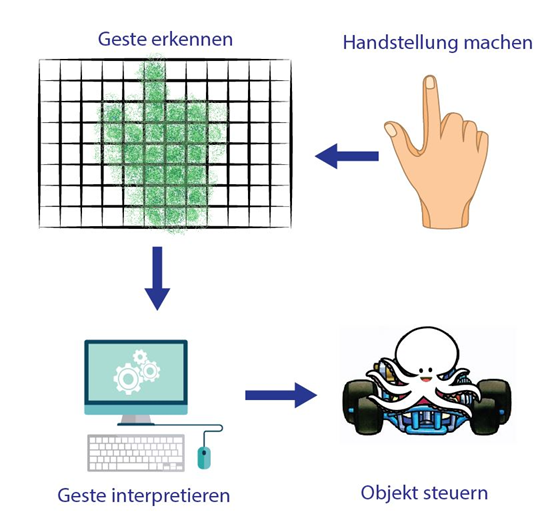
\includegraphics[scale=0.8]{figures/AblaufGestikulaser.png}
	\caption{\textcolor{red}{Erklärung!}}
	\label{fig:AblaufGestikulaser}
\end{figure}

Der Gestikulaser selbst besteht aus einer Platte, der Photoplatte, welche aus verschiedenen Steckmodulen zusammen gesteckt werden kann. Die Steckmodule bestehen aus einzelnen kleinen Boxen, in welche die Elektronik integriert ist. In der Mitte befindet sich der Oktokommander, welcher durch weitere Detektormodule erweitert werden kann. Auf jedes der Module befinden sich vier Photodioden um das reflektierte Licht zu messen. 

\begin{figure}[h]
	\centering
	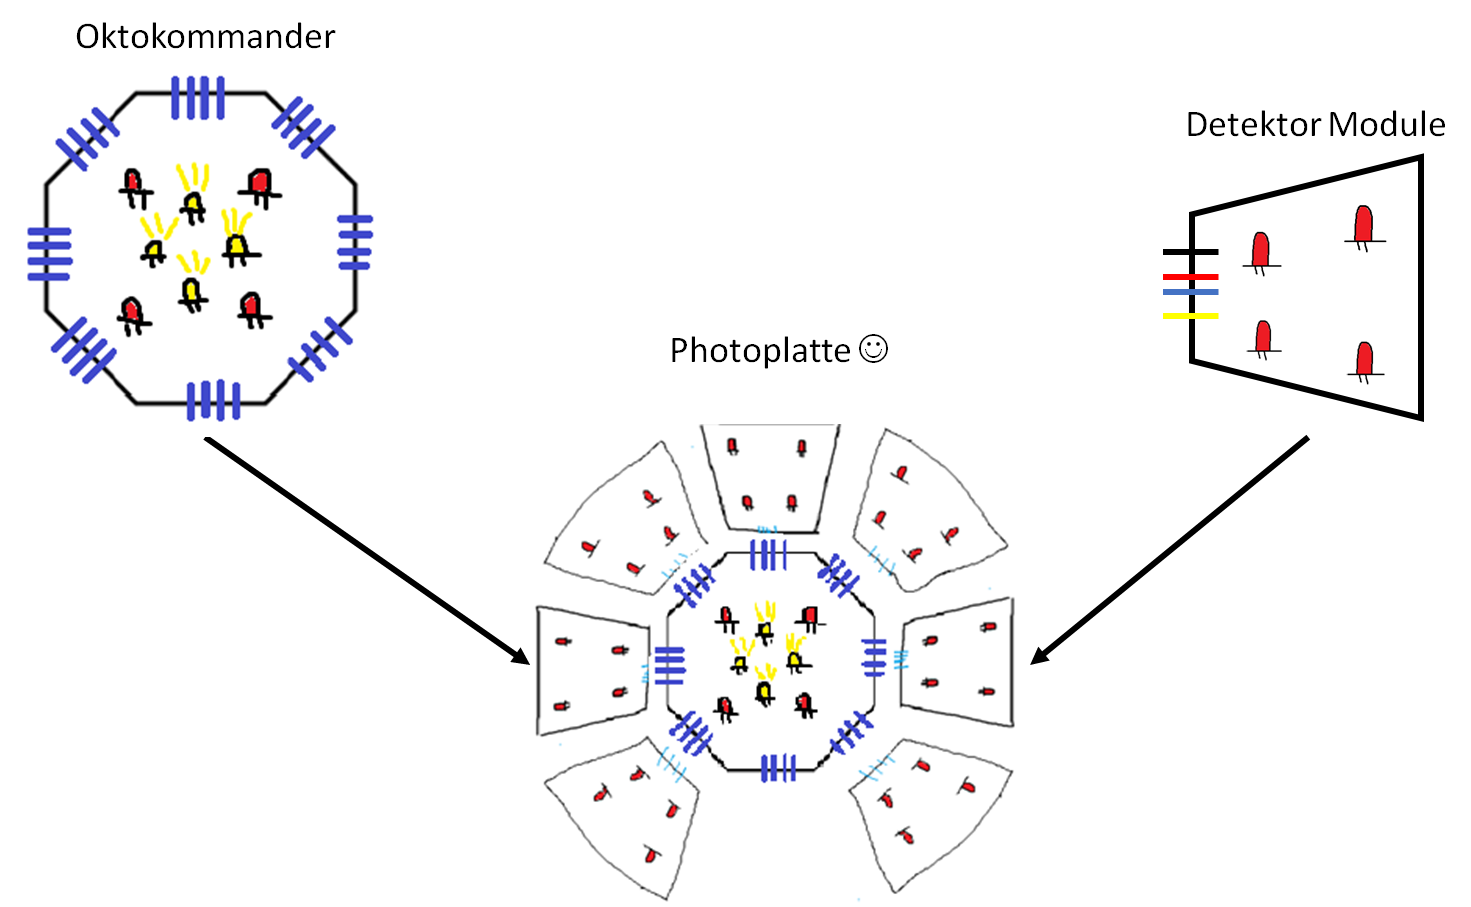
\includegraphics[scale=0.5]{figures/Photoplatte.png}
	\caption{\textcolor{red}{Erklärung!}}
	\label{fig:Fotoplatte}
\end{figure}

% -------------------------------------------------------------------------------------- %

\section{Oktokommander}
\label{sec:Oktokommander}

Der Oktokommander ist das Steuersystem der gesamten Photoplatte. In ihr befinden sich ein Arduino Micro, welcher die Signale aller Photodioden bearbeitet sowie einen i2c Expander. Durch den i2c Expander ist es möglich, jedes der Photodioden eine eigene Adresse zu zu weisen. Dies ist nötig, um die voneinander unabhängigen Signale der Photodioden richtig zuordnen zu können. Zusätzlich dazu befinden sich auf dem Oktokommander vier Infrarot LEDs sowie vier infrarot Photodioden. Um die vier infrarot Photodioden an zu steuern wird zusätzlich zum i2c Expander noch ein i2c Multiplexer sowie die dazu gehörende Verstärkerschaltung benötigt. 
\textcolor{red}{Erklärung der Komponenten an Hand des Bildes}

\begin{figure}[h]
	\centering
	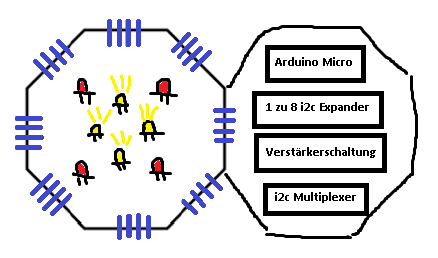
\includegraphics[scale=0.8]{figures/OktokommanderOffen.png}
	\caption{\textcolor{red}{Erklärung!}}
	\label{fig:OktokommanderOffen}
\end{figure}

Um den Oktokommander mit den Detektormodulen erweitern zu können wurden USB-2A Schnittstellen verwendet. Durch diese Schnittstellen können bis zu 7 Detektormodule, jeweils eines pro Seite  eingekoppelt werden. Um eine größere Platte zu konstruieren können noch weitere Detektormodule an den bereits vorhandenen Detektormodule angeschlossen werden.
\textcolor{red}{Erklärung der Komponenten an Hand des Bildes}

\begin{figure}[h]
	\centering
	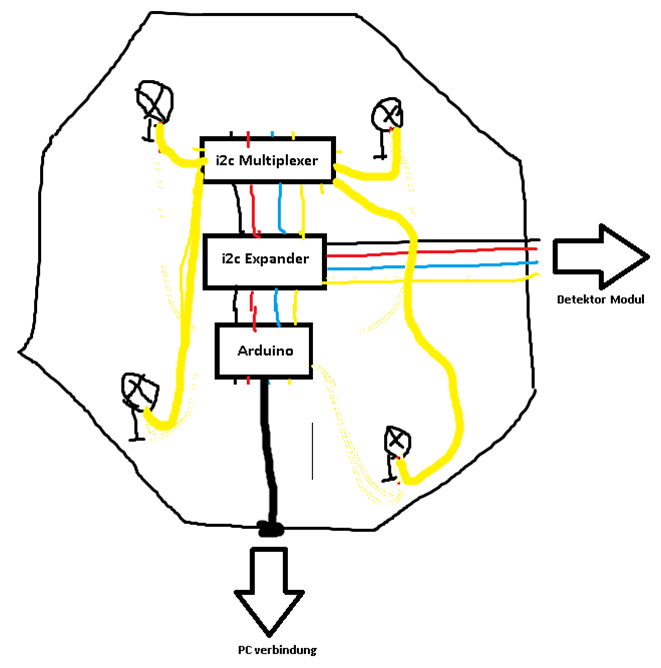
\includegraphics[scale=0.8]{figures/PrinzipskizzeOktokommander.png} 
	\caption{\textcolor{red}{Erklärung!}}
	\label{fig:PrinzipskizzeOktokommander}
\end{figure}

% -------------------------------------------------------------------------------------- %

\section{Detektormodul}
\label{sec:Detektormodul}

Das Detektormodul besteht lediglich aus vier Photodioden und einem USB-2A Eingang. Dadurch kann das Detektormodul an den Oktokommander angeschlossen werden. Zur Ansteuerung der Photodioden wurde auch hier ein i2c Expander verwendet. 
\textcolor{red}{Erklärung der Komponenten der Bilder}

\begin{figure}[h]
	\centering
	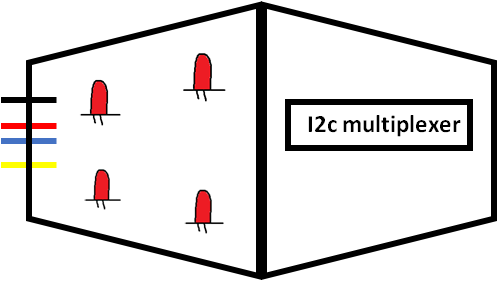
\includegraphics[scale=0.7]{figures/DetektormodulOffen.png}
	\caption{\textcolor{red}{Erklärung!}}
	\label{fig:DetektormodulOffen}
\end{figure}

\begin{figure}[h]
	\centering
	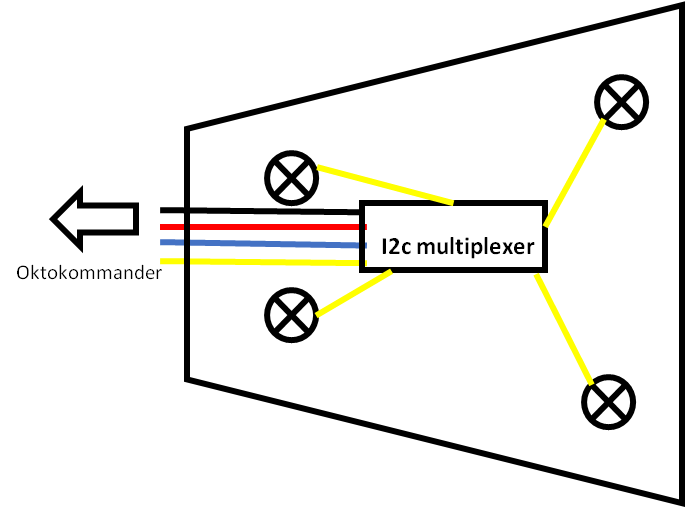
\includegraphics[scale=0.5]{figures/PrinzipskizzeDetektormodul.png}
	\caption{\textcolor{red}{Erklärung!}}
	\label{fig:PrinzipskizzeDetektormodul}
\end{figure}

% -------------------------------------------------------------------------------------- %

\section{Software}
\label{sec:Software}


\chapter{Marketing und Kosten}
\label{ch:Kosten}

Neben der Entwicklung unseres Produktes wurde im Laufe der Entwicklungszeit zusätzliche Öffentlichkeitsarbeiten geleistet. So wurde die Website \url{https://www.gestikulaser.de/} ins Leben gerufen sowie der Instagram Account \href{https://www.instagram.com/laserharptos/}{\texttt{laserharptos}} mit über 100 Abonnenten betreut. 
Im Zuge dessen wurde auch Sponsoren angeworben, welche Interesse an der Unterstützung unseres Projektes hatten. \\

Folgende Sponsoren haben uns bei diesem Projekt unterstützt: \\

\begin{tabularx}{\textwidth}{r c}
	Aconity3D GmbH & \noindent\parbox[c]{\hsize}{
\includegraphics[scale=0.07]{../Logos/AC3D_Logo_Print-for-white.png}} \\
	& \\
	Fraunhofer ILT & \noindent\parbox[c]{\hsize}{
\includegraphics[scale=0.1]{../Logos/Fraunhofer_ILT.png}} \\
	& \\
	TOS RWTH Aachen University & \noindent\parbox[c]{\hsize}{
\includegraphics[scale=0.5]{../Logos/TOS.png}} \\
	\vspace{1.5cm} & \\
	Würth Electronik GmbH \& Co. KG & \noindent\parbox[c]{\hsize}{
\includegraphics[scale=0.05]{../Logos/Wuerth.png}}
\end{tabularx} \\

Die Produktionskosten unseres Gestikulasers können wie folgt aufgegliedert werden:\\

\large{\underline{\textbf{Oktokommander}}} \\ 

\normalsize
\begin{tabularx}{\textwidth}{p{4.5cm} | c c c c}

Produktname 			& Kosten /Stk 		& Anzahl & Gesamtkosten    & Kostenträger \\ \hline
Arduino Micro 			& $19.99$ \euro{}   &   1    & $19.99$ \euro{} & TOS 	\\ [2mm]
I2C-Multiplexer TCA9548A& $7.80$ \euro{}    &   1    & $7.80$ \euro{}  & ILT    \\ [8mm]
I2C ADS1015				& $11.20$ \euro{}   &   1    & $11.20$ \euro{} & ILT    \\ [2mm]
Infrarot LED    		&					&   4    &				   & Würth  \\ [2mm]
LED Treiber     		&                   &   2    &                 & Würth  \\ [2mm]
Infrarot Photodiode 	&					&   4    &                 & ILT	\\ [8mm] 
OP-Verstärker    		& $1.85$ \euro{}    &	4    & $7.40$ \euro{}  & TOS    \\ [2mm]
UBS 2 TypA -Mount		&                   &   7    &                 & Würth  \\ [2mm]
Passive Bauteile    	&	---------       &   ---  &	$1$ \euro{}	   & TOS    \\ [2mm]\hline
						&					&		 & $  60  $	\euro{}&

\end{tabularx}\\

\large{\underline{\textbf{Detektormodul}}} \\ 

\normalsize
\begin{tabularx}{\textwidth}{p{4.5cm} | c c c c}

Produktname 			& Kosten /Stk 		& Anzahl & Gesamtkosten    & Kostenträger \\ \hline
I2C ADS1015				& $11.20$ \euro{}   &   1    & $11.20$ \euro{} & ILT    \\ [2mm]
Infrarot Photodiode 	&					&   4    &                 & ILT	\\ [8mm]
OP-Verstärker    		& $1.85$ \euro{}    &	4    & $7.40$ \euro{}  & TOS    \\ [2mm]
UBS 2 TypA -Plug		&                   &   1    &                 & Würth  \\ [2mm]
UBS 2 TypA -Mount		&                   &   1    &                 & Würth  \\ [2mm]
Passive Bauteile    	&	-----  	        &	-	 &	$1$ \euro{}	   & TOS    \\ [2mm]\hline
						&					&		 & $  20  $	\euro{}&
					
\end{tabularx} \\

Dabei wurde ein Oktokommander und sieben Detektormodule aufgebaut. Die Gesamtkosten für die Produktion belaufen sich also auf 200€.\\

Darüber hinaus sind Kosten von BLA \euro{} für Unterkunft und Anreise entstanden sowie T-Shirts in Wert von BLA \euro{}. Die T-Shirts wurden von Aconity3D gespondert.

\appendix

\chapter{Ausblick}
\label{ch:Ausblick}

\textcolor{red}{Erweiterung um Sensorhandschuh zur verbesserten Erkennung der Daten. Überarbeitung des Designs um die Module besser bzw. anders zusammen zu stecken.}

\end{document}